\subsection{Kennlinien der Hochvakuumdiode} 
Aus den Tabellen (\ref{taba1} - \ref{taba5}) sind die darauf folgenden 
Abbildungen (\ref{pica1} - \ref{pica5}) erstellt worden.
\begin{table}[h!]
	\begin{center}
		\begin{tabular}{cc}
			Anodenspannung [V] & Anodenstrom [mA]\\ \hline
			10	&0,044\\
			20	&0,088\\
			30	&0,108\\
			40	&0,119\\
			50	&0,126\\
			60	&0,128\\
			70	&0,132\\
			80	&0,135\\
			90	&0,138\\
			100	&0,141\\
			110	&0,144\\
			120	&0,146\\
			130	&0,147\\
			140	&0,149\\
			150	&0,150\\
			160	&0,151\\
			170	&0,152\\
			180	&0,154\\
			190	&0,155\\
			200	&0,156\\
			210	&0,157
		\end{tabular}
		\caption{Kennlinie 1 (Heizwerte: 4,2V; 2,1A)}
		\label{taba1}
	\end{center}
\end{table} \begin{table}[h]
	\begin{center}
		\begin{tabular}{cc}
			Anodenspannung [V] & Anodenstrom [mA]\\ \hline
			10	&0,049\\
			20	&0,123\\
			30	&0,181\\
			40	&0,232\\
			50	&0,263\\
			60	&0,281\\
			70	&0,302\\
			80	&0,310\\
			90	&0,322\\
			100	&0,330\\
			110	&0,336\\
			120	&0,340\\
			130	&0,344\\
			140	&0,348\\
			150	&0,352\\
			160	&0,355\\
			170	&0,359\\
			180	&0,362\\
			190	&0,366\\
			200	&0,368\\
			210	&0,371\\
			220	&0,373\\
			230	&0,375\\
			240	&0,377\\
			250	&0,380
		\end{tabular}
		\caption{Kennlinie 2 (Heizwerte: 4,8V; 2,2A)}
		\label{taba2}
	\end{center}
\end{table} \begin{table}[h]
	\begin{center}
		\begin{tabular}{cc}
			Anodenspannung [V] & Anodenstrom [mA]\\ \hline
			10	&0,050\\
			20	&0,135\\
			30	&0,230\\
			40	&0,309\\
			50	&0,367\\
			60	&0,421\\
			70	&0,479\\
			80	&0,525\\
			90	&0,555\\
			100	&0,589\\
			110	&0,622\\
			120	&0,642\\
			130	&0,655\\
			140	&0,665\\
			150	&0,671\\
			160	&0,677\\
			170	&0,682\\
			180	&0,686\\
			190	&0,692\\
			200	&0,697\\
			210	&0,702\\
			220	&0,706\\
			230	&0,709\\
			240	&0,713\\
			250	&0,717
		\end{tabular}
		\caption{Kennlinie 3 (Heizwerte: 5,0V; 2,3A)}
		\label{taba3}
	\end{center}
\end{table} \begin{table}[h]
	\begin{center}
		\begin{tabular}{cc}
			Anodenspannung [V] & Anodenstrom [mA]\\ \hline
			10	&0,061\\
			20	&0,163\\
			30	&0,275\\
			40	&0,383\\
			50	&0,460\\
			60	&0,575\\
			70	&0,689\\
			80	&0,812\\
			90	&0,947\\
			100	&1,042\\
			110	&1,131\\
			120	&1,229\\
			130	&1,343\\
			140	&1,452\\
			150	&1,566\\
			160	&1,666\\
			170	&1,779\\
			180	&1,882\\
			190	&1,984\\
			200	&2,08\\
			210	&2,18\\
			220	&2,28\\
			230	&2,37\\
			240	&2,45\\
			250	&2,53
		\end{tabular}
		\caption{Kennlinie 4 (Heizwerte: 5,9V; 2,5A)}
		\label{taba4}
	\end{center}
\end{table} \begin{table}[h]
	\begin{center}
		\begin{tabular}{cc}
			Anodenspannung [V] & Anodenstrom [mA]\\ \hline
			10	&0,063\\
			20	&0,170\\
			30	&0,288\\
			40	&0,398\\
			50	&0,514\\
			60	&0,606\\
			70	&0,711\\
			80	&0,829\\
			90	&0,958\\
			100	&1,107\\
			110	&1,282\\
			120	&1,399\\
			130	&1,494\\
			140	&1,593\\
			150	&1,730\\
			160	&1,865\\
			170	&2,00\\
			180	&2,14\\
			190	&2,29\\
			200	&2,44\\
			210	&2,58\\
			220	&2,72\\
			230	&2,86\\
			240	&3,00\\
			250	&3,11
		\end{tabular}
		\caption{Kennlinie 5 (Heizwerte: 6,1V; 2,6A)}
		\label{taba5}
	\end{center}
\end{table}
	\begin{figure}[h]
		\begin{center}
		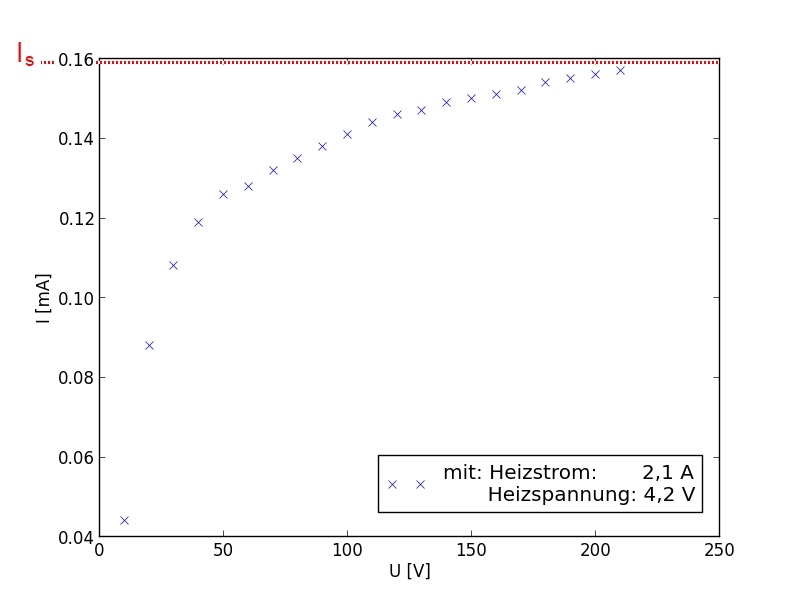
\includegraphics[scale=0.75]{pica1.jpg}
		\caption{Kennlinie 1 (Heizwerte: 4,2V; 2,1A)}
		\label{pica1}
		\end{center}	
	\end{figure} 	\begin{figure}[h]
		\begin{center}
		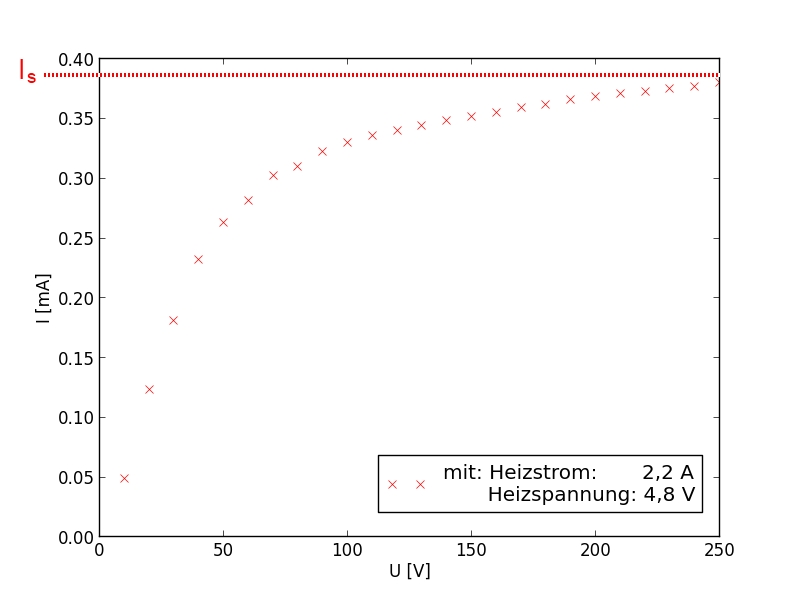
\includegraphics[scale=0.75]{pica2.jpg}
		\caption{Kennlinie 2 (Heizwerte: 4,8V; 2,2A)}
		\label{pica2}
		\end{center}	
	\end{figure} 	\begin{figure}[h]
		\begin{center}
		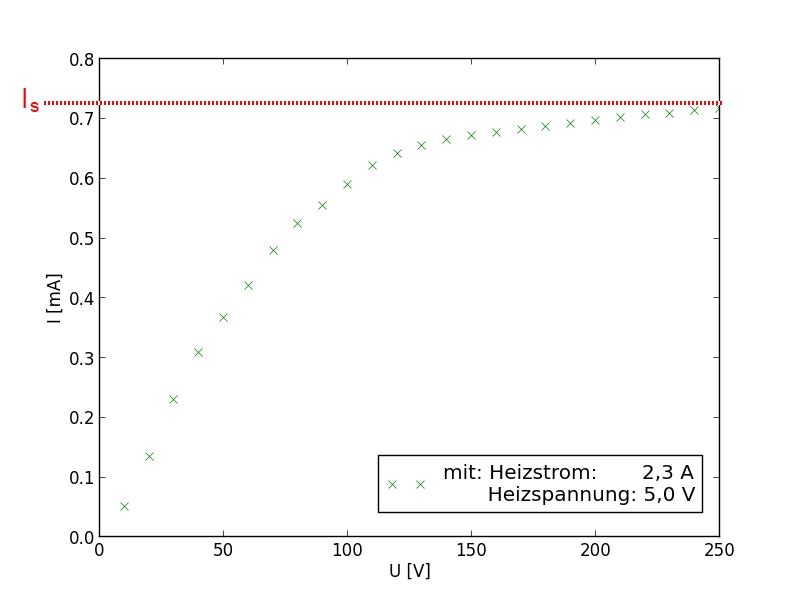
\includegraphics[scale=0.75]{pica3.jpg}
		\caption{Kennlinie 3 (Heizwerte: 5,0V; 2,3A)}
		\label{pica3}
		\end{center}	
	\end{figure} 	\begin{figure}[h]
		\begin{center}
		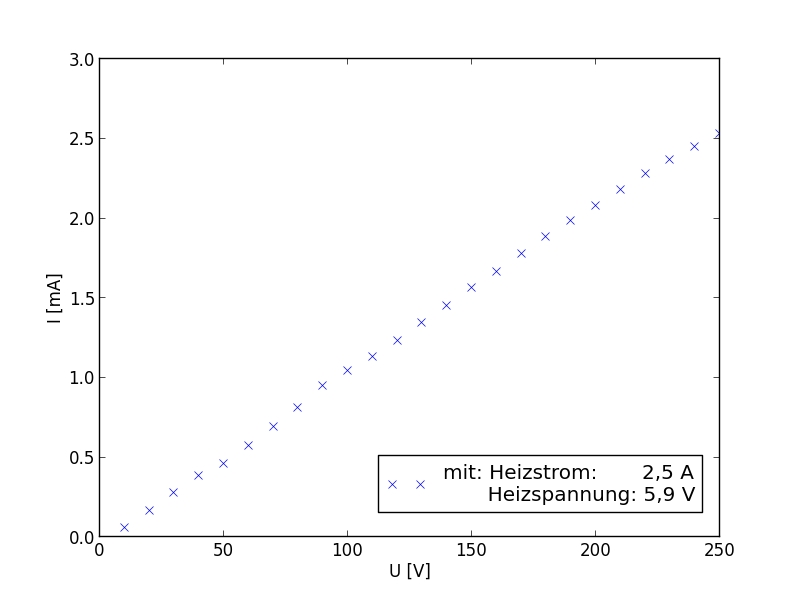
\includegraphics[scale=0.75]{pica4.jpg}
		\caption{Kennlinie 4 (Heizwerte: 5,9V; 2,5A)}
		\label{pica4}
		\end{center}	
	\end{figure} 	\begin{figure}[h]
		\begin{center}
		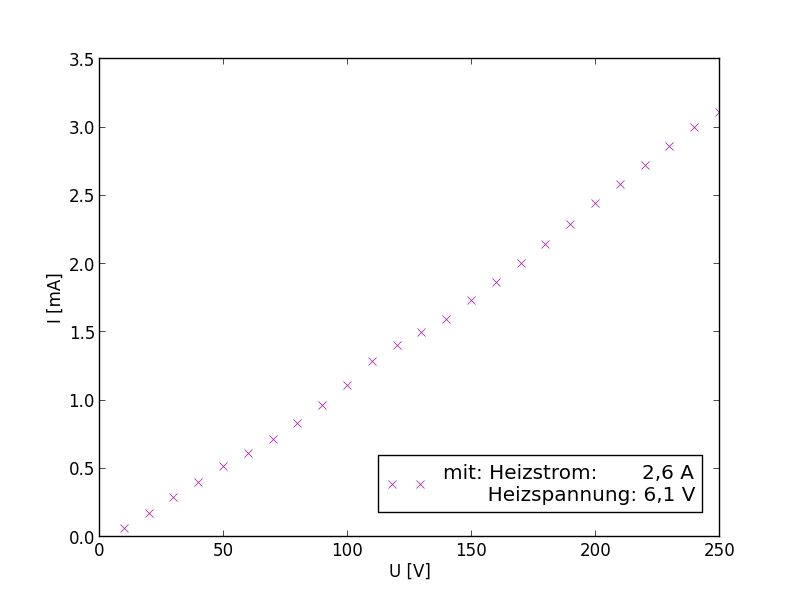
\includegraphics[scale=0.75]{pica5.jpg}
		\caption{Kennlinie 5 (Heizwerte: 6,1V; 2,6A)}
		\label{pica5}
		\end{center}	
	\end{figure} 
Aus den Abbildungen \ref{pica1},\ref{pica2} und \ref{pica3} wurde der Sättingungsstrom 
$I_s$ abgelesen (Tab. \ref{tabis}). Bei den Abbildungen \ref{pica4} und \ref{pica5} war das 
nicht möglich, der Großteil des Sättigungsstromgebietes befand sich außerhalb der 
Messwerte.
\begin{table}[h]
	\begin{center}
		\begin{tabular}{ccc}
			Heizspannung [V] & Heizstrom [A] & Sättigungsstrom [mA]\\ \hline
			4,2 &2,1 &0,16\\
			4,8 &2,2 &0,38\\
			5,0 &2,3 &0,72
		\end{tabular}
		\caption{Sättigungstromwerte}
		\label{tabis}
	\end{center}
\end{table}
\FloatBarrier
\subsection{Langmuir-Schottkysches-Gesetz}
Das Langmuir-Schottkysche Raumladungsgesetz (Gl. \ref{eqlangmuir}) ist solange gültig, bis sich die Kennlinie
dem Sättigungstrom annähert, also das Raumladungsgebiet in das Sättigungsstromgebiet 
übergeht. Für die maximal mögliche Heizleistung passiert das ungefähr bei 200V.
Trägt man die Messwerte logarithmisch auf, so lässt sich der Exponent erkennen (vgl. 
Abb. \ref{picb1}). Der Exponent berechnet sich durch lineare Regression \cite{linreg}
aus Gleichung \ref{eqb1}, beziehungsweise Tabelle \ref{tabblinreg}, welche auf Tabelle \ref{taba5} aufbaut.
\begin{align}
I&\sim U^\alpha \\
\Rightarrow ln(I)&\sim ln(U)*\alpha \label{eqb1}
\end{align}
\begin{table}[h]
	\begin{center}
		\begin{tabular}{cccc}
			U[V] & I[mA] & ln(U) & ln(I)\\ \hline
			10	&0,063& 2,30& -2,765\\                  
			20	&0,170& 2,99& -1,772\\
			30	&0,288& 3,40& -1,245\\
			40	&0,398& 3,68& -0,921\\
			50	&0,514& 3,91& -0,666\\
			60	&0,606& 4,09& -0,501\\
			70	&0,711& 4,24& -0,341\\
			80	&0,829& 4,38& -0,188\\
			90	&0,958& 4,49& -0,043\\
			100	&1,107& 4,60& 0,102\\
			110	&1,282& 4,70& 0,248\\
			120	&1,399& 4,78& 0,336\\
			130	&1,494& 4,86& 0,402\\
			140	&1,593& 4,94& 0,466\\
			150	&1,730& 5,01& 0,548\\
			160	&1,865& 5,07& 0,623\\
			170	&2,000& 5,13& 0,693\\
			180	&2,140& 5,19& 0,761\\
			190	&2,290& 5,24& 0,829\\
		\end{tabular}
		\caption{Logarithmen zur Kennlinie 5 (Heizwerte: 6,1V; 2,6A)}
		\label{tabblinreg}
	\end{center}
\end{table}
\FloatBarrier
Aus der linearen Regression nach \cite{linreg} berechnet sich der gesuchte Exponent $\alpha$ beziehungsweise die Ausgleichskurve (Abb. \ref{picb1}).
\begin{align}
y&=a*x+b \\
\Leftrightarrow ln(I)&=1,1808*ln(U)-5,3443 \\
a&=\alpha=1,1808 \label{exalpha}\\
\Delta a&=1,24\% \\
b&=-5.3443 \\
\Delta b&=1,22\% \\
\Rightarrow I&=U^\alpha*e^b 
\end{align}
	\begin{figure}[h]
		\begin{center}
		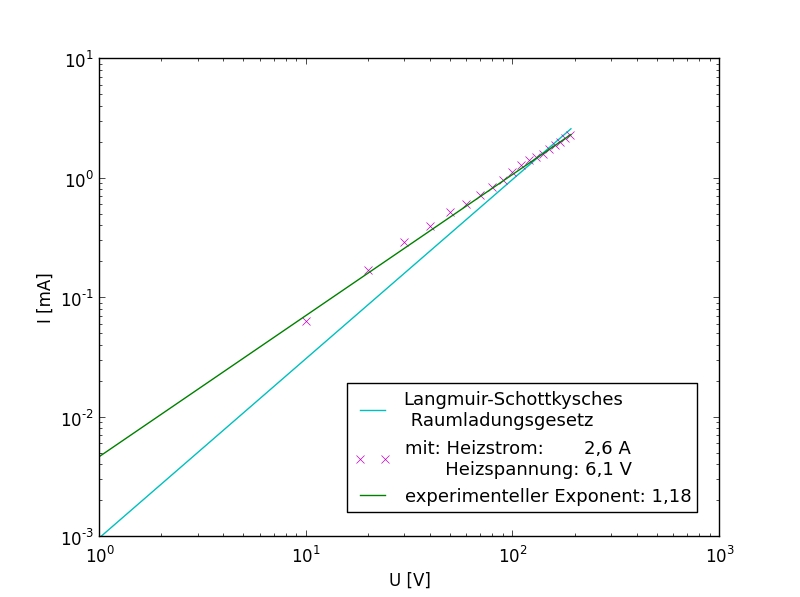
\includegraphics[scale=0.75]{picb1.jpg}
		\caption{Strom-Spannungs-Beziehung}
		\label{picb1}
		\end{center}	
	\end{figure}
\FloatBarrier
\subsection{Kathodentemperatur im Anlaufstromgebiet}
Aus den aufgezeichneten Messwerten (vgl. Tab. \ref{tabc1}) lässt sich nach der Gleichung \ref{eqcureal}
die angezeigte Spannung $U_{Heiz}$ nach $U_{Heiz,real}$ korrigieren. Daraus lässt sich dann mit 
Gleichung \ref{eqtemp} T berechnen (Tab. \ref{tabc1}). Die genutzen Apparaturkonstanten waren dabei:
\begin{align}
\begin{split}
f&=0,335cm^2 \label{eqdatatemp}\\
\eta&=0,28\\
N_{WL}&=0,95W .
\end{split}
\end{align} 
Die Werte sind in Abbildung \ref{picc1} veranschaulicht.
\begin{align}
U_a'&=U_a+R*I_a\\
\Rightarrow U_{Heiz,real}&=U_{Heiz}-R*I_S \label{eqcureal}\\
mit: R&=1M\Omega
\end{align}
\begin{table}[h]
	\begin{center}
		\begin{tabular}{cc}
			$U_{gegen}$ [V]&$I_{Anlauf}$ [nA] \\ \hline
			0,0&115,00\\
			0,1&91,00\\
			0,2&65,00\\
			0,3&44,50\\
			0,4&30,00\\
			0,5&20,00\\
			0,6&12,50\\
			0,7&7,50\\
			0,8&4,50\\
			0,9&2,90\\
			1,0&1,65
		\end{tabular}
		\caption{Anlaufstromgebiet (Heizwerte: 6,1V; 2,6A)}
		\label{tabcdata}
	\end{center}
\end{table}
\begin{table}[h]
	\begin{center}
		\begin{tabular}{cc}
			$6{,}1V-U_{Heiz,real}$[$\mu$V]&2298K-T[$\mu$K] \\ \hline
			0,11&207 \\
			0,091&205\\
			0,065&202\\
			0,045&200\\
			0,030&199\\
			0,020&198\\
			0,013&197\\
			0,0075&197\\
			0,0045&196\\
			0,0029&196\\
			0,0017&196
		\end{tabular}
		\caption{Kathodentemperatur im Anlaufstromgebiet($U_{Heiz}=6,1V$)}
		\label{tabc1}
	\end{center}
\end{table} 	\begin{figure}[h]
		\begin{center}
		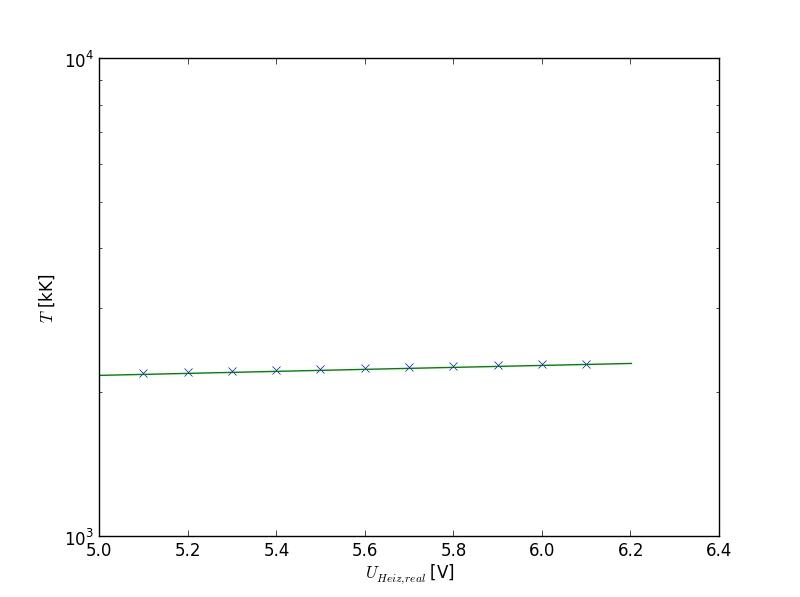
\includegraphics[scale=0.75]{picc1.jpg}
		\caption{Kathodentemperatur im Anlaufstromgebiet}
		\label{picc1}
		\end{center}	
	\end{figure}
\FloatBarrier
\subsection{Kathodentemperatur bei Saugspannung}
Die Leistungbilanz des Heizstromkreises dient nach Gleichung \ref{eqtemp} mit den Werten aus \ref{eqdatatemp}
zur Berechnung der Temperatur aus den aufgezeichneten Werten (vgl. Tab. \ref{taba1}-\ref{taba5}). Die Ergebnisse
sind in Tabelle \ref{tabd1} und in Abbildung \ref{picd1} dargestellt. 
\begin{table}[h]
	\begin{center}
		\begin{tabular}{cc}
			U[V]&$\Delta Q [\frac{\text{C}}{e}] * 10^9$ \\ \hline
			339&63,68\\
			342&11,50\\
			345&13,53\\
			348&12,40\\
			351&13,25\\
			354&12,39\\
			357&11,92\\
			360&12,01\\
			410&18,17\\
			460&24,10\\
			510&30,09\\
			560&35,97\\
			610&41,55\\
			650&47,73\\
			653&48,29\\
			656&46,66\\
			659&48,33\\
			662&46,36\\
			665&52,44\\
			668&52,20\\
			671&52,79\\
			674&53,75\\
			677&50,56\\
			680&51,58\\
			683&50,60\\
			686&54,91\\
			689&49,79\\
			692&48,88\\
			695&50,28\\
			698&46,15\\
			701&52,62
		\end{tabular}
		\caption{freigesetzte Ladungsmenge im Zählrohr}
		\label{tabd1}
	\end{center}
\end{table} 	\begin{figure}[h]
		\begin{center}
		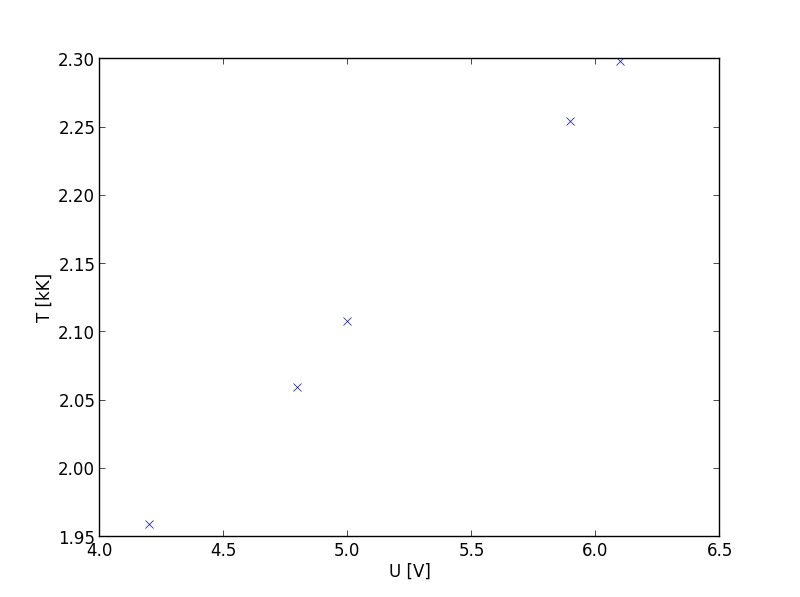
\includegraphics[scale=0.75]{picd1.jpg}
		\caption{Kathodentemperatur unter Heizleistungsvariation}
		\label{picd1}
		\end{center}	
	\end{figure}
\FloatBarrier
\subsection{Austrittsarbeit des Kathodenmaterials}
Um die Austrittsarbeit der Wolfram-Kathode nach der Richardson-Gleichung \ref{eqrichard} zu berechnen,
werden die T Werte aus Tabelle \ref{tabd1} und die Sättigungsstromwerte aus Tabelle \ref{tabis}
verwendet. Die Ergebnisse für die Austrittsarbeit $e_o\varphi$ sind in Tabelle \ref{tabe1} zusammengefasst.
Der Mittelwert der Austrittsarbeit $\overline{e_o\varphi}$, welcher nach Gleichung \ref{eqmittwert} berechnet
wird, beträgt:
\begin{align}
\overline{e_o\varphi}&=6{,}5\overline{3} \label{eqphi} \\
\overline{x}&=\frac{1}{N}\sum\limits_{i=1}^N x_i \label{eqmittwert}
\end{align}
\begin{table}[h]
	\begin{center}
		\begin{tabular}{cc}
			$I_S$[mA]& $e_0\varphi$[eV] \\ \hline
			0,16&4,71\\
			0,38&4,81\\
			0,72&4,82\\
			2,80&4,91\\
			3,50&4,97
		\end{tabular}
		\caption{Austrittsarbeit (Wolfram)}
		\label{tabe1}
	\end{center}
\end{table}
\FloatBarrier

